\subsection{Bidirectional Interfaces}

{\em Bidirectional interfaces\/} % enable us to
model components that have bidirectional connections. 
% Unlike in Moore interfaces, where a state of the interface consists 
% simply of an assignment of values to input and output variables, 
% in bidirectional interfaces we find it convenient to have an
% additional set $Q$ of locations. 
To model bidirectionality we find it convenient to add to the Moore model
a set $Q$ of {\em locations}.
% Informally, a bidirectional interface works as follows. 
Informally, each location $q \in Q$ partitions the interface variables 
into inputs and outputs, and determines what values are legal for 
the inputs, and what values can be assigned to the outputs. 
% determines which variables are used as outputs,
% and which are used as inputs, by the interface. 
% The location $q$ also determines what values are legal for 
% the inputs, and which values can be assigned to the outputs. 
% Once the values for the variables used as outputs and inputs have been
% chosen by the interface and its environments, these values determine
% the successor $q' \in Q$ of $q$.
At each location $q \in Q$, a particular choice of output and input 
values determines the successor location $q'$. 
The precise definition is as follows. 

\begin{defi}{(Bidirectional interfaces)}
A \emph{bidirectional interface} $\mp$ is a tuple 
$\tuple{\vars_\mp,Q_\mp,\hat{q}_\mp,\ovarsf_\mp,\phi^i_\mp,\phi^o_\mp,\trel_\mp}$
consisting of the following components: 
%
\begin{itemize}
\item A finite set $\vars_\mp$ of input or output {\em (inout)} variables.

\item A finite set $Q_\mp$ of locations, including an initial location
$\hat{q}_\mp \in Q_\mp$.

\item A function $\ovarsf_\mp: Q_\mp \rightarrow 2^{\vars_\mp}$, that
associates with all $q \in Q_\mp$ the set $\ovarsf_\mp(q)$ of variables
that are used as outputs at location $q$.
For all $q \in Q_\mp$, 
we denote by $\ivarsf_\mp(q) = \vars_\mp \setm \ovarsf_\mp(q)$ the set
of variables that are used as inputs.

\item Two labelings $\phi^i_\mp$ and $\phi^o_\mp$, which associate with
each location $q \in Q_\mp$ a predicate $\phi^i_\mp(q)$ on $\ivarsf_\mp(q)$, called 
the input assumption, and a predicate $\phi^o_\mp(q)$ on $\ovarsf_\mp(q)$,
called the output guarantee. 
% Luca: for homogeneity, we always want a successor. 
% A location $q \in Q_\mp$ is a {\em termination location} if the output
% guarantee $\phi^o_\mp(q)$ is unsatisfiable.  
% A location $q \in Q_\mp$ is an {\em error location} if the input assumption
% $\phi^i_\mp(q)$ is unsatisfiable but the output guarantee $\phi^o_\mp(q)$
% is satisfiable.  
For all $q \in Q_\mp$, both $\phi^i_\mp(q)$ and $\phi^o_\mp(q)$ should be
satisfiable. 

\item A labeling $\rho_\mp$, which associates with each pair of locations
$q,r \in Q_\mp$ a predicate $\rho_\mp(q,r)$ on $\vars_\mp$,
called the {\em transition guard.}
We require that for every location $q \in Q_\mp$, (i)~the disjunction
$\bigvee_{r \in Q_\mp}\rho_\mp(q,r)$ is valid and (ii)~$\forall r, r'
\in Q_\mp$, $(r \neq r') \Rightarrow \lnot (\rho_\mp(q,r) \land
\rho_\mp(q,r'))$.
Condition~(i)  ensures that the interface is non-blocking, and
condition~(ii) ensures determinism. 
% Luca: I am not using this.  Is it used? 
% If $\rho_\mp(q,r)$ is satisfied by a valuation $s$ on $\ovarsf_\mp(q) \cup
% \ivarsf_\mp(q)$, then $r$ is called a $s$-successor of $q$ and denoted
% $\delta_\mp(q,s)$. 
\qed 

\end{itemize}
\end{defi}

\noindent 
We let 
$\ivars_\mp = \bigcup_{q \in Q_\mp} \ivarsf_\mp(q)$ and 
$\ovars_\mp = \bigcup_{q \in Q_\mp} \ovarsf_\mp(q)$
be the sets of all variables that are ever used as inputs or outputs
(note that we do not require $\ivars_\mp \inters \ovars_\mp = \emptyset$). 
% Given $p,q \in Q_\mp$, we say that $q$ is {\em reachable from $p$ in one
% step\/} if $\phi^i_\mp(p) \und \phi^o_\mp(p) \und \rho_\mp(p,q)$ is
% satisfiable, and we say that $p$ is {\em reachable\/} from $q$ if
% there is a sequence $p = p_0, p_1, \ldots, p_k = q$ where $p_{j+1}$ is
% reachable from $p_j$ in one step for $0 \leq j < k$. 
We define the set
$\traces(\tuple{\vars_\mp,Q_\mp,\hat{q}_\mp,\phi^i_\mp,\phi^o_\mp,\trel_\mp})$ 
of {\em bidirectional traces\/} to be the set of infinite sequences 
$q_0, s_0, q_1, s_1, \ldots$, where $q_0 = \hat{q}_\mp$, 
and for all $k \geq 0$, we have 
$q_k \in Q_\mp$,  $s_k \in \states[\vars_\mp]$, and 
$s_k \sat (\phi^i_\mp(q_k) \und \phi^o_\mp(q_k) \und \trel_\mp(q_k,q_{k+1}))$.
For $q_0, s_0, q_1, s_1, \ldots \in
\traces(\tuple{\vars_\mp,Q_\mp,\hat{q}_\mp,\phi^i_\mp,\phi^o_\mp,\trel_\mp})$
and $k \geq 0$, we say that $q_k$ is {\em reachable\/} in 
$\tuple{\vars_\mp,Q_\mp,\hat{q}_\mp,\phi^i_\mp,\phi^o_\mp,\trel_\mp}$. 

\noindent
Composition of bidirectional interfaces is defined along the
same lines as for Moore interfaces. % Informally, now 
Local 
incompatibilities arise not only when one interface output values 
do not satisfy the input assumptions of the other, but also when 
the same variable is used as output by both interfaces. The formal 
definition follows.
%\mynote{cut?}
% Again, two interfaces $\mp$ and $\mq$ are compatible (written
% $\mp\compat\mq$) if we can
% strengthen the input assumptions of their composition to ensure that
% no such local incompatibilities occur; 
% we associate with the composition the weakest such input assumptions,
% and we prune the locations that become unreachable as a result of the
% strengthening.
% The algorithm for computing the input assumptions of the composition 
% starts by strengthening the input assumptions to ensure that the input
% assumptions of the composed interfaces are satisfied. 
% As this may create locations with unsatisfiable input assumptions
% (``illegal locations'') we then iteratively strengthen the input
% assumptions of all locations, until such error locations are no longer
% reachable.

\begin{defi}{(Composition of bidirectional interfaces)}
\label{def-ag-comp} 
\newline
Given two bidirectional interfaces 
$\mp$ and $\mq$, let 
$\vars_\oprod = \vars_\mp \union \vars_\mq$, 
$Q_\oprod = Q_\mp \times Q_\mq$, 
and $\hat{q}_\oprod = (\hat{q}_\mp,\hat{q}_\mq)$. 
For all $(p,q) \in Q_\mp \times Q_\mq$, 
let $\phi^o_\oprod(p,q) = \phi^o_\mp(p) \und \phi^o_\mp(q)$,  
and for all $(p',q') \in Q_\mp \times Q_\mq$, let 
$\trel_\oprod ((p,q), (p',q')) = \trel_\mp (p,p') \und \trel_\mq(p,p')$. 
The interfaces $\mp$ and $\mq$ are {\em compatible\/} 
(written $\mp \compat \mq$) if there is a
labeling $\psi$ associating with all $(p,q) \in Q_\oprod$ 
a predicate $\psi(p,q)$ on 
$\vars_\oprod \setm (\ovars_\mp(p) \union \ovars_\mq(q))$ such that 
(i)~$\psi(p,q)$ is satisfiable at all $(p,q) \in Q_\oprod$, and 
(ii) all traces $(p_0,q_0), s_0, (p_1,q_1), s_1, (p_2,q_2), s_2, \ldots \in 
\traces(\vars_\oprod, Q_\oprod, \hat{q}_\oprod, 
\psi, \phi^o_\oprod,\trel_\oprod)$ 
satisfy, for all $k \geq 0$, the conditions 
(a)~$\ovars_\mp(p_k) \inters \ovars_\mq(q_k) = \emptyset$ and 
(b)~$s_k \sat \phi^i_\mp(p_k) \und \phi^i_\mq(q_k)$. 
The composition $\mr = \mp \| \mq$  is defined if and only if 
$\mp$ and $\mq$ are compatible; if they are, then $\mr = \mp \| \mq$
is obtained by taking for $\phi^i_\mr$ the weakest predicate $\psi$ 
such that the above conditions (a) and (b) on traces hold,
by taking for $Q_\mr$ the subset of locations of $Q_\oprod$ 
that are reachable in 
$\tuple{\vars_\oprod,Q_\oprod,\hat{q}_\oprod,\ovars_\oprod,
\phi^i_\mr,\phi^o_\oprod,\trel_\oprod}$, 
by taking $\vars_\mr = \vars_\oprod$ 
and $\hat{q}_\mr = \hat{q}_\oprod$, 
and by taking for $\ovars_\mr,\phi^i_\mr,\phi^o_\mr$, and $\trel_\mr$ 
the restrictions of 
$\ovars_\oprod,\phi^i_\oprod,\phi^o_\oprod$, and $\trel_\oprod$ 
to $Q_\mr$. 
\qed
\end{defi}

% \noindent
% As for Moore interfaces, composition of bidirectional 
% interfaces is thus a partial function, and is associative. The
% following algorithm computes the composition.
%: 
% for all bidirectional interfaces $\mp$, $\mq$, $\mr$, 
% either $(\mp \| \mq) \| \mr$ and 
% $(\mp \| \mq) \| \mr$ are both undefined (due to incompatibilities), 
% or they are both defined. 
% In this latter case,  $(\mp \| \mq) \| \mr$ and $(\mp \| \mq) \| \mr$
% are equal, up to isomorphism of the location graph. 

\begin{algo}{}
\label{algo-ag-comp} 
Given two bidirectional interfaces $\mp$ and $\mq$, let 
$\vars_\oprod = \vars_\mp \union \vars_\mq$, 
$Q_\oprod = Q_\mp \times Q_\mq$, 
and $\hat{q}_\oprod = (\hat{q}_\mp,\hat{q}_\mq)$. 
For all $(p,q) \in Q_\mp \times Q_\mq$, 
let $\phi^i_\oprod(p,q) = \phi^i_\mp(p) \und \phi^i_\mp(q)$,  
and for all $(p',q') \in Q_\mp \times Q_\mq$, let 
$\trel_\oprod ((p,q), (p',q')) = \trel_\mp (p,p') \und \trel_\mq(p,p')$. 
The input labeling $\phi^i_\oprod(p,q)$ is computed by repeating the
following steps, that progressively strengthen the input assertions: 
%
\begin{quote}
[Step 1] For all $(p,q) \in Q_\mp \times Q_\mq$, 
if $\ovarsf_\mp(p) \inters \ovarsf_\mq(q) \neq \emptyset$, 
then initialize $\phi^i_\oprod(p,q)$ to $\false$; 
otherwise initialize $\phi^i_\oprod(p,q)$ to the predicate 
$\forall \ovarsf_\oprod (p,q) . 
  (\phi^o_\oprod (p,q) \im (\phi^i_\mp (p) \und \phi^i_\mq (q))$. 

\medskip \noindent 
[Step 2]
For all $(p,q)$ and $(p',q')$ in $Q_\mp \times Q_\mq$, 
if $\phi^i_\oprod(p',q')$ is unsatisfiable, then replace 
$\phi^i_\oprod(p,q)$ with 
$\phi^i_\oprod(p,q) \und \forall \ovarsf_\oprod (p,q) . 
  (\phi^o_\oprod (p,q) \im \no \rho_\oprod((p,q),(p',q'))$. 

\medskip \noindent 
Repeat [Step 2] until all input assumptions are replaced by equivalent
predicates, i.e., are not strengthened. 

\end{quote}
%
We have that $\mp \compat \mq$ iff 
$\phi^i_\oprod(\hat{q}_\mp,\hat{q}_\mq)$ is satisfiable.  
If $\mp\compat\mq$ then their composition $\mr$ is defined by taking
$Q_\mr$ to be the subset of locations of $Q_\oprod$ that are reachable
in  
$\tuple{\vars_\oprod,Q_\oprod,\hat{q}_\oprod,\ovarsf_\oprod,
\phi^i_\mr,\phi^o_\oprod,\trel_\oprod}$, 
by taking $\vars_\mr = \vars_\oprod$ 
and $\hat{q}_\mr = \hat{q}_\oprod$, 
and by taking for $\ovarsf_\mr,\phi^i_\mr,\phi^o_\mr$, and $\trel_\mr$ 
the restrictions of 
$\ovarsf_\oprod,\phi^i_\oprod,\phi^o_\oprod$, and $\trel_\oprod$ 
to $Q_\mr$.
\qed
\end{algo}

\noindent
We have developed and implemented symbolic algorithms for composition and 
compatibility and refinement checking of bidirectional interfaces.
The tool, written in Java, is based on the CUDD Package used in
JMocha \cite{Mocha2001}. 
In our implementation, the locations are represented
explicitly, while the input assumptions and output guarantees at each
location are represented and manipulated symbolically. 
This hybrid representation is well-suited to the modeling of
bidirectional interfaces, where the set of input and output
variables depends on the location. 

\begin{figure}[tb]
\centering
% \subfigure[PCI Local Bus Structural Diagram]{\label{pcistr}
\subfigure[]{\label{pcistr}
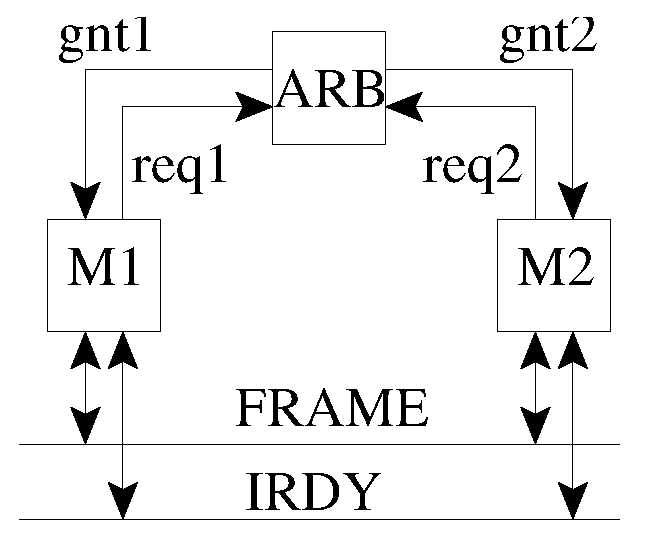
\includegraphics[scale=0.27]{pcistr.eps}}  % arindam: please do not delete this line. used for fig2ps
% \input{pcistr}}
% \subfigure[PCI Master Interface]{\label{pcistate}
\hspace{0.11in}
\subfigure[]{\label{pcistate}
% \includegraphics[scale=0.18]{pcistate.pstex}}  arindam: please do not delete this line. used for fig2ps
\begin{picture}(0,0)%
\includegraphics{pcistate.ps}%
\end{picture}%
\setlength{\unitlength}{1066sp}%
%
\begingroup\makeatletter\ifx\SetFigFont\undefined%
\gdef\SetFigFont#1#2#3#4#5{%
  \reset@font\fontsize{#1}{#2pt}%
  \fontfamily{#3}\fontseries{#4}\fontshape{#5}%
  \selectfont}%
\fi\endgroup%
\begin{picture}(6317,5739)(151,-5860)
\put(4951,-2761){\makebox(0,0)[lb]{\smash{\SetFigFont{8}{9.6}{\rmdefault}{\mddefault}{\updefault}{\color[rgb]{0,0,0}$\lnot$}%
}}}
\put(4276,-3511){\makebox(0,0)[lb]{\smash{\SetFigFont{8}{9.6}{\rmdefault}{\mddefault}{\updefault}{\color[rgb]{0,0,0}$\top$}%
}}}
\put(4276,-3886){\makebox(0,0)[lb]{\smash{\SetFigFont{8}{9.6}{\rmdefault}{\mddefault}{\updefault}{\color[rgb]{0,0,0}$\top$}%
}}}
\put(1276,-1861){\makebox(0,0)[lb]{\smash{\SetFigFont{8}{9.6}{\rmdefault}{\mddefault}{\updefault}{\color[rgb]{0,0,0}$\top$}%
}}}
\put(2476,-4786){\makebox(0,0)[lb]{\smash{\SetFigFont{8}{9.6}{\rmdefault}{\mddefault}{\updefault}{\color[rgb]{0,0,0}$\land$}%
}}}
\put(2401,-3061){\makebox(0,0)[lb]{\smash{\SetFigFont{8}{9.6}{\rmdefault}{\mddefault}{\updefault}{\color[rgb]{0,0,0}$\lnot$}%
}}}
\put(2251,-436){\makebox(0,0)[lb]{\smash{\SetFigFont{8}{9.6}{\rmdefault}{\mddefault}{\updefault}{\color[rgb]{0,0,0}$\lnot$}%
}}}
\put(1276,-1336){\makebox(0,0)[lb]{\smash{\SetFigFont{8}{9.6}{\rmdefault}{\mddefault}{\updefault}{\color[rgb]{0,0,0}$\lnot$}%
}}}
\put(526,-3961){\makebox(0,0)[lb]{\smash{\SetFigFont{8}{9.6}{\rmdefault}{\mddefault}{\updefault}{\color[rgb]{0,0,0}$\top$}%
}}}
\put(526,-4336){\makebox(0,0)[lb]{\smash{\SetFigFont{8}{9.6}{\rmdefault}{\mddefault}{\updefault}{\color[rgb]{0,0,0}$\top$}%
}}}
\put(226,-5611){\makebox(0,0)[lb]{\smash{\SetFigFont{8}{9.6}{\rmdefault}{\mddefault}{\updefault}{\color[rgb]{0,0,0}$\land$}%
}}}
\put(601,-5611){\makebox(0,0)[lb]{\smash{\SetFigFont{8}{9.6}{\rmdefault}{\mddefault}{\updefault}{\color[rgb]{0,0,0}$\lnot$}%
}}}
\end{picture}
}
\hspace{0.11in}
% \subfigure[Composition of two PCI master interfaces]{\label{pcicompstate}
\subfigure[]{\label{pcicompstate}
\includegraphics[scale=0.27]{pcicompstate.eps}} \\ % arindam: please do not delete this line. used for fig2ps
% \input{pcicompstate}}
% \subfigure[Token-ring NT interface]{\label{tokenringstate}
\subfigure[]{\label{tokenringstr}
\includegraphics[scale=0.27]{tokenringstr.eps}}  % arindam: please do not delete this line; needed for fig2ps
% \input{tokenringstr}}
\hspace{0.15in}
\subfigure[]{\label{tokenringstate}
% \includegraphics[scale=0.18]{tokenringstate.pstex}}  arindam: please do not delete this line; needed for fig2ps
\begin{picture}(0,0)%
\includegraphics{tokenringstate.ps}%
\end{picture}%
\setlength{\unitlength}{1066sp}%
%
\begingroup\makeatletter\ifx\SetFigFont\undefined%
\gdef\SetFigFont#1#2#3#4#5{%
  \reset@font\fontsize{#1}{#2pt}%
  \fontfamily{#3}\fontseries{#4}\fontshape{#5}%
  \selectfont}%
\fi\endgroup%
\begin{picture}(7734,6264)(601,-5635)
\put(976,-4636){\makebox(0,0)[lb]{\smash{\SetFigFont{8}{9.6}{\rmdefault}{\mddefault}{\updefault}{\color[rgb]{0,0,0}$\top$}%
}}}
\put(901,-4186){\makebox(0,0)[lb]{\smash{\SetFigFont{8}{9.6}{\rmdefault}{\mddefault}{\updefault}{\color[rgb]{0,0,0}$\lnot$}%
}}}
\put(1276,-3661){\makebox(0,0)[lb]{\smash{\SetFigFont{8}{9.6}{\rmdefault}{\mddefault}{\updefault}{\color[rgb]{0,0,0}$\land$}%
}}}
\put(901,-2386){\makebox(0,0)[lb]{\smash{\SetFigFont{8}{9.6}{\rmdefault}{\mddefault}{\updefault}{\color[rgb]{0,0,0}$\lnot$}%
}}}
\put(901,-661){\makebox(0,0)[lb]{\smash{\SetFigFont{8}{9.6}{\rmdefault}{\mddefault}{\updefault}{\color[rgb]{0,0,0}$\lnot$}%
}}}
\put(901,-1036){\makebox(0,0)[lb]{\smash{\SetFigFont{8}{9.6}{\rmdefault}{\mddefault}{\updefault}{\color[rgb]{0,0,0}$\lnot$}%
}}}
\put(1501,239){\makebox(0,0)[lb]{\smash{\SetFigFont{8}{9.6}{\rmdefault}{\mddefault}{\updefault}{\color[rgb]{0,0,0}$\lnot$}%
}}}
\put(6976,-586){\makebox(0,0)[lb]{\smash{\SetFigFont{8}{9.6}{\rmdefault}{\mddefault}{\updefault}{\color[rgb]{0,0,0}$\top$}%
}}}
\put(6976,-961){\makebox(0,0)[lb]{\smash{\SetFigFont{8}{9.6}{\rmdefault}{\mddefault}{\updefault}{\color[rgb]{0,0,0}$\lnot$}%
}}}
\put(6151,-3361){\makebox(0,0)[lb]{\smash{\SetFigFont{8}{9.6}{\rmdefault}{\mddefault}{\updefault}{\color[rgb]{0,0,0}$\lnot$}%
}}}
\put(6976,-4186){\makebox(0,0)[lb]{\smash{\SetFigFont{8}{9.6}{\rmdefault}{\mddefault}{\updefault}{\color[rgb]{0,0,0}$\lnot$}%
}}}
\put(6976,-4561){\makebox(0,0)[lb]{\smash{\SetFigFont{8}{9.6}{\rmdefault}{\mddefault}{\updefault}{\color[rgb]{0,0,0}$\lnot$}%
}}}
\put(5476,-5536){\makebox(0,0)[lb]{\smash{\SetFigFont{8}{9.6}{\rmdefault}{\mddefault}{\updefault}{\color[rgb]{0,0,0}$\lnot$}%
}}}
\put(5101,314){\makebox(0,0)[lb]{\smash{\SetFigFont{8}{9.6}{\rmdefault}{\mddefault}{\updefault}{\color[rgb]{0,0,0}$\lnot$}%
}}}
\put(6526,314){\makebox(0,0)[lb]{\smash{\SetFigFont{8}{9.6}{\rmdefault}{\mddefault}{\updefault}{\color[rgb]{0,0,0}$\land$}%
}}}
\put(6976,-2761){\makebox(0,0)[lb]{\smash{\SetFigFont{8}{9.6}{\rmdefault}{\mddefault}{\updefault}{\color[rgb]{0,0,0}$\lnot$}%
}}}
\put(7126,-1561){\makebox(0,0)[lb]{\smash{\SetFigFont{8}{9.6}{\rmdefault}{\mddefault}{\updefault}{\color[rgb]{0,0,0}$\land$}%
}}}
\put(1801,-5461){\makebox(0,0)[lb]{\smash{\SetFigFont{8}{9.6}{\rmdefault}{\mddefault}{\updefault}{\color[rgb]{0,0,0}$\land$}%
}}}
\put(2176,-5536){\makebox(0,0)[lb]{\smash{\SetFigFont{8}{9.6}{\rmdefault}{\mddefault}{\updefault}{\color[rgb]{0,0,0}$\lnot$}%
}}}
\put(1501,-1711){\makebox(0,0)[lb]{\smash{\SetFigFont{8}{9.6}{\rmdefault}{\mddefault}{\updefault}{\color[rgb]{0,0,0}$\lnot$}%
}}}
\end{picture}
}

\caption{PCI and Token-ring Protocols 
\ref{pcistr} PCI Local Bus Structural Diagram
\ref{pcistate} PCI Master Interface
\ref{pcicompstate} Composite interface for two PCI Master Modules
\ref{tokenringstr} Token Ring Network Configuration
\ref{tokenringstate} Token-ring NT Interface
} 
\end{figure}

\begin{examp}{(PCI Bus)}
% The PCI bus protocol is well-known and widely used. 
We consider a PCI
bus configuration with two PCI-compliant master devices and a PCI
arbiter as shown in Figure~\ref{pcistr}.
Each PCI master device has an $gnt$ input and a $req$ output to
communicate with the arbiter, and a set of shared (read-write)
signals, the \verb+IRDY+ and the \verb+FRAME+, which are used to 
communicate with target devices. 
% The arbiter has the responsibility of deciding which master device is
% allowed to write to the shared signals in a bus cycle; more than one
% master writing simultaneously to the shared signals would be an error.
The arbiter ensures that at most one master device can 
write to the shared signals.
Figure~\ref{pcistate} shows a graphical description of the interface
representing a master device. The figure shows for each location, the
assumption (``a''), the guarantee (``g''), the set of inout variables 
that the interface writes to, and guarded transitions between locations.
Composing two such interfaces we obtain the interface shown in 
Figure~\ref{pcicompstate}. Location \verb+Owner_Owner+ is illegal
because both components write the shared variables \verb+FRAME+ and 
\verb+IRDY+. Input assumptions of locations \verb+Req_Req+, 
\verb+Owner_Req+ and \verb+Req_Owner+ are strengthened to make the 
illegal location unreachable.
Note that this propagates the PCI master's assumptions 
about its environment to an assumption on the behavior of the arbiter 
(which is the environment of the composite module): 
the arbiter should never assert \verb+gnt1+ (\verb+gnt2+) during or
after asserting \verb+gnt2+ (\verb+gnt1+),  until \verb+req2+
(\verb+req1+) is de-asserted at least once. \qed 
\end{examp}

\subsection{Properties of compatibility and composition} 

If $\mp$ and $\mq$ are composable Moore interfaces, we define their
{\em product\/} $\mp\oprod\mq$ by 
$\ovars_{\mp\oprod\mq} = \ovars_\mp \union \ovars_\mq$ and
$\ivars_{\mp\oprod\mq} = 
	(\ivars_\mp \union \ivars_\mq) \setm \ovars_{\mp\oprod\mq}$, 
and by letting 
$\oinit_{\mp\oprod\mq} = \oinit_\mp \und \oinit_\mq$, 
$\iinit_{\mp\oprod\mq} = \iinit_\mp \und \iinit_\mq$, 
$\otrans_{\mp\oprod\mq} = \otrans_\mp \und \otrans_\mq$, and 
$\itrans_{\mp\oprod\mq} = \otrans_\mp \und \itrans_\mq$.
\begin{comment} 
Intuitively, an environment for a Moore interface $\mp$ is an
interface that drives all free inputs of $\mp$, ensuring that all the
input assumptions are met. 
Precisely, we say that a Moore interface $\mq$ is an 
{\em environment\/} for a Moore interface $\mp$ if 
(i)~$\mp$ and $\mq$ are composable;
(ii)~$\mp\prod\mq$ is closed i.e., $\ivars_{\mp\oprod\mq} =
\emptyset$; 
(iii)~$\mp\prod\mq$ is non-blocking, i.e., $\iinit_{\mp\oprod\mq}$ is
satisfiable, and $\forall \ovars_{\mp\oprod\mq} . (\exists
\ivars_{\mp\oprod\mq})' . \itrans_{\mp\oprod\mq}$ holds; and 
(iv)~for all sequences $s_0, s_1, s_2, \ldots$ of
states in $\states[\vars_{\mp\oprod\mq}]$ with $s_0 \sat
\oinit_{\mp\oprod\mq}$ and $(s_k,s_{k+1}) \sat \otrans_{\mp\oprod\mq}$
for all $k \geq 0$, we have also that $s_0 \sat \iinit_{\mp\oprod\mq}$
and $(s_k,s_{k+1}) \sat \itrans_{\mp\oprod\mq}$ for all $k \geq 0$.
\end{comment}
%
Intuitively, an {\em environment\/} for a Moore interface $\mp$ is an
interface that drives all free inputs of $\mp$, ensuring that all the
input assumptions are met. 
Precisely, we say that a Moore interface $\mq$ is an 
environment for a Moore interface $\mp$ if $\mp$ and $\mq$ are
composable and closed (i.e., $\ovars_\mp \inters \ovars_\mq =
\emptyset$, and $\ivars_{\mp\oprod\mq} = \emptyset$), and if the
following conditions hold:  

%\vspace*{-1ex}

\begin{itemize}
\item {\em Non-blocking:\/} $\iinit_{\mp\oprod\mq}$ is satisfiable,
and $\forall \ovars_{\mp\oprod\mq} . (\exists \ivars_{\mp\oprod\mq})'
. \itrans_{\mp\oprod\mq}$ holds. 
\item {\em Legal:\/} for all sequences $s_0, s_1, s_2, \ldots$ of
states in $\states[\vars_{\mp\oprod\mq}]$ with $s_0 \sat
\oinit_{\mp\oprod\mq}$ and $(s_k,s_{k+1}) \sat \otrans_{\mp\oprod\mq}$
for all $k \geq 0$, we have also that $s_0 \sat \iinit_{\mp\oprod\mq}$
and $(s_k,s_{k+1}) \sat \itrans_{\mp\oprod\mq}$ for all $k \geq 0$.
\end{itemize}

%\vspace*{-1ex}

\noindent
Analogous definitions for product and environment can be given for
bidirectional interfaces. 
The following theorem states the main properties of compatibility and
composition of Moore interfaces; an analogous result holds for
bidirectional interfaces. 

\begin{theo}{(properties of compatibility and composition)}
The following assertions hold: 
%
\begin{enumerate}

\item % {\em Associativity:\/} 
Given three Moore interfaces $\mp$,
$\mq$, $\mr$, either $(\mp \| \mq) \| \mr$ and $(\mp \| \mq) \| \mr$
are both undefined (due to non-composability or incompatibility), or
they are both defined, in which case they are equal.

\item % {\em Compatibility as existence of environment:\/}
Given two composable Moore interfaces $\mp$ and $\mq$, we have that $\mp
\compat \mq$ iff there is an environment for $\mp\oprod\mq$. 

\item % {\em Composition and input assumptions:\/} 
Given two compatible Moore interfaces $\mp$ and $\mq$, 
and $\mr$ composable with $\mp\|\mq$, 
we have that $(\mp\|\mq) \compat \mr$ iff there is an environment 
for $\mp\oprod\mq\oprod\mr$. 

\end{enumerate}
\end{theo}

\noindent
The second assertion makes precise our statement that two interfaces
are compatible iff there is some environment in which they can work
correctly together. 
The third assertion states that composition does not unduly restrict
the input assumptions: checking compatibility with the composition
$\mp\|\mq$ amounts to checking compatibility with $\mp$ and $\mq$. 


